\chapter{Analyse van Observatieprestaties}
\label{ch:analyse}

\section{Inleiding}

In de voorgaande hoofdstukken werden de ontwikkeling van de PoC applicatie, de methodologie voor het verzamelen 
van experimentele data, en het creëren van een grondwaarheidsdataset uitvoerig besproken. 
Dit hoofdstuk richt zich op de kern van het onderzoek: de geautomatiseerde analyse van de 
observatieprestaties van studenten aan de hand van de verzamelde eyetracking-opnames.

Het hoofddoel van de hier beschreven analyse is om, op basis van de videofeed en blikdata van de Tobii Pro Glasses 3, 
utomatisch te bepalen (1) welke van de vooraf gedefinieerde kritische objecten door een student zijn waargenomen en (2) 
hoe lang de aandacht op elk van deze objecten gericht was. 
Om dit te realiseren, werd een analysepipeline ontworpen en geïmplementeerd, die de output van verschillende computervisiemodellen combineert.

Hier worden de componenten van deze analysepipeline in detail toegelicht, beginnend met een initiële `segment everything' stap, 
gevolgd door filtering op basis van blikdata en objectgrootte, en culminerend in de classificatie van de relevante objectsegmenten. 
Er worden twee verschillende benaderingen voor de classificatiestap geëvalueerd: één op basis van image embeddings (DINOv2) en een vector-index (Faiss), 
en een tweede die gebruikmaakt van een getraind YOLO-classificatiemodel. 
De prestaties van deze methoden zullen worden beoordeeld aan de hand van de in Hoofdstuk~\ref{ch:grondwaarheid} gecreëerde grondwaarheid.

\subsection{Analysepipeline}

De ontwikkelde analysepipeline, zoals conceptueel voorgesteld in Strategie 4 van Hoofdstuk~\ref{ch:oplossingsstrategieen}, 
bestaat uit een reeks opeenvolgende stappen die een inputframe uit een eyetracking-opname transformeren naar een geclassificeerd, bekeken object. 
Figuur~\ref{fig:analyse-pipeline-visualisatie} illustreert de fasen van dit proces aan de hand van representatieve beelden.

\begin{figure}[H]
    \centering
        \begin{subfigure}[b]{0.75\textwidth}
        \centering
        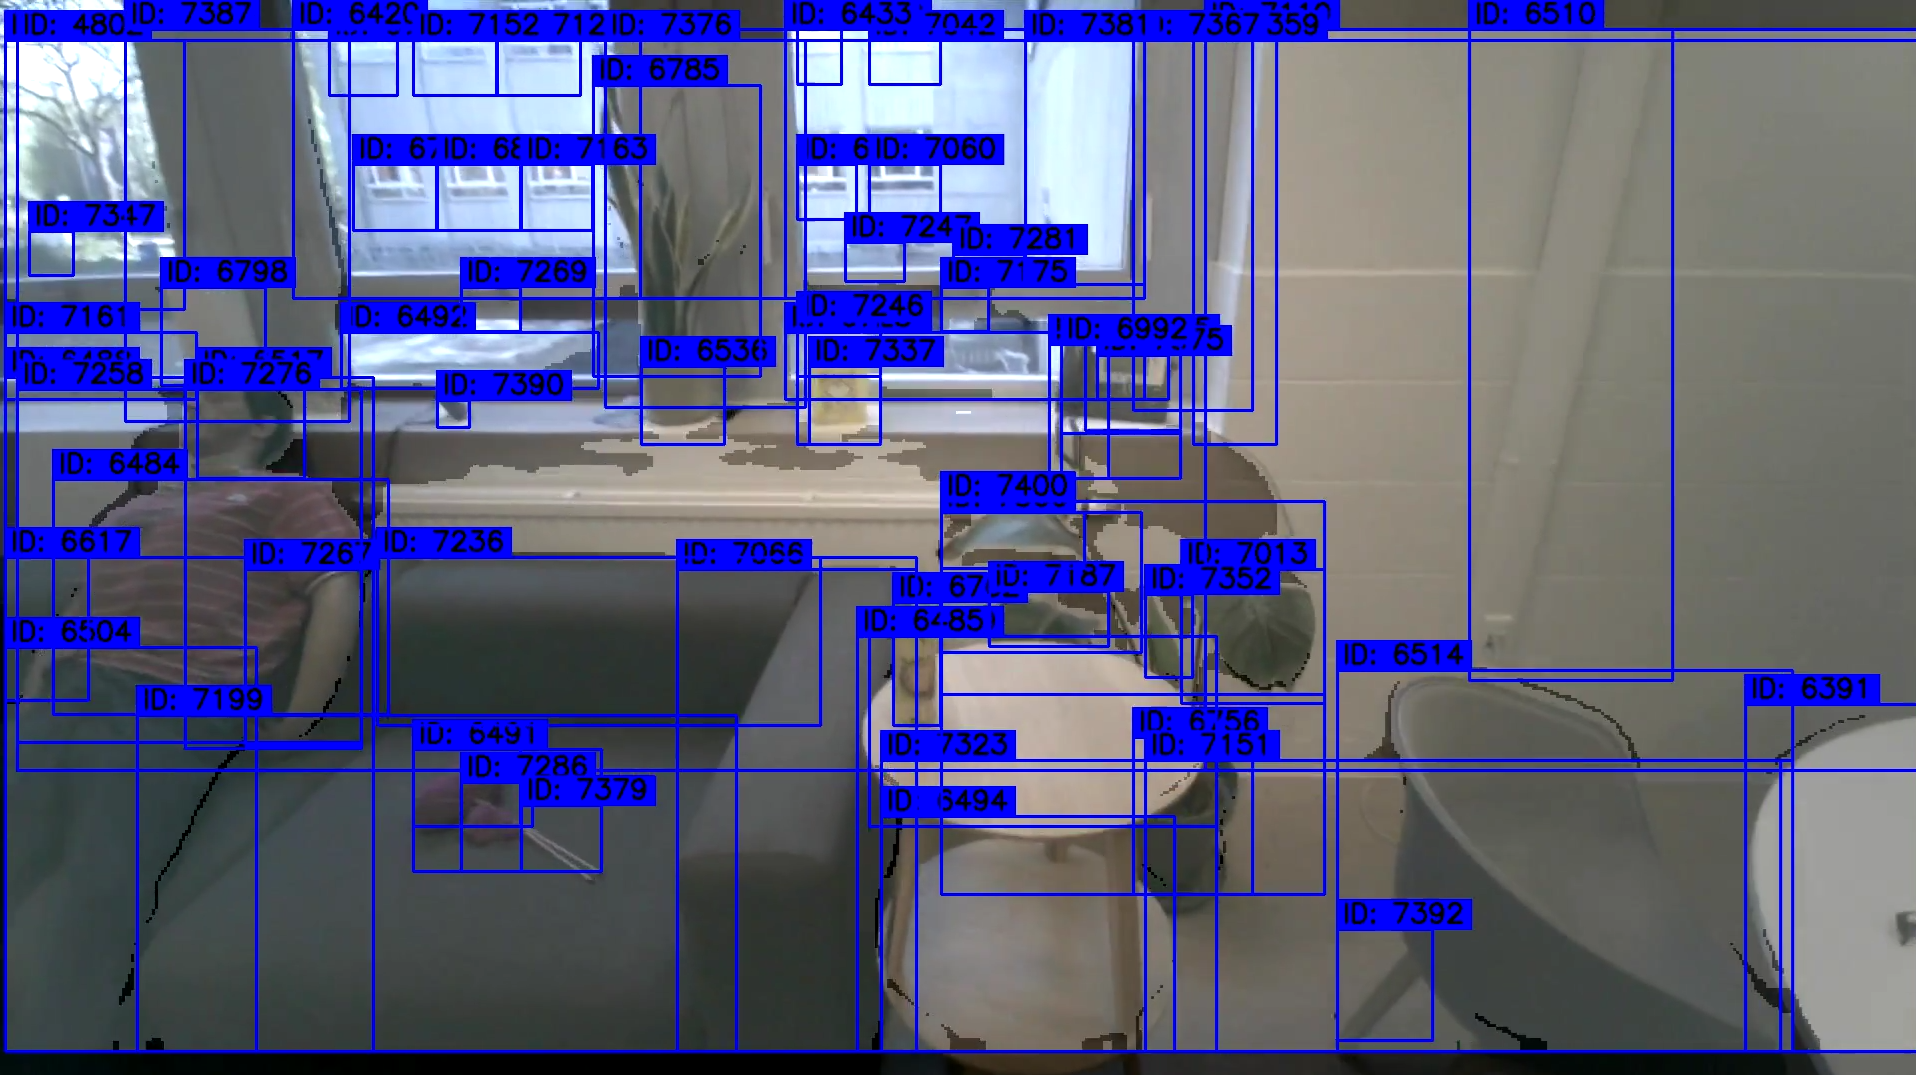
\includegraphics[width=1\textwidth]{everything-prompt.png}
        \caption{Everything-Segmentatie (FastSAM)}
        \label{fig:pipeline_stap_a}
    \end{subfigure}

    \vspace{0.5cm}

    \begin{subfigure}[b]{0.75\textwidth}
    \centering
    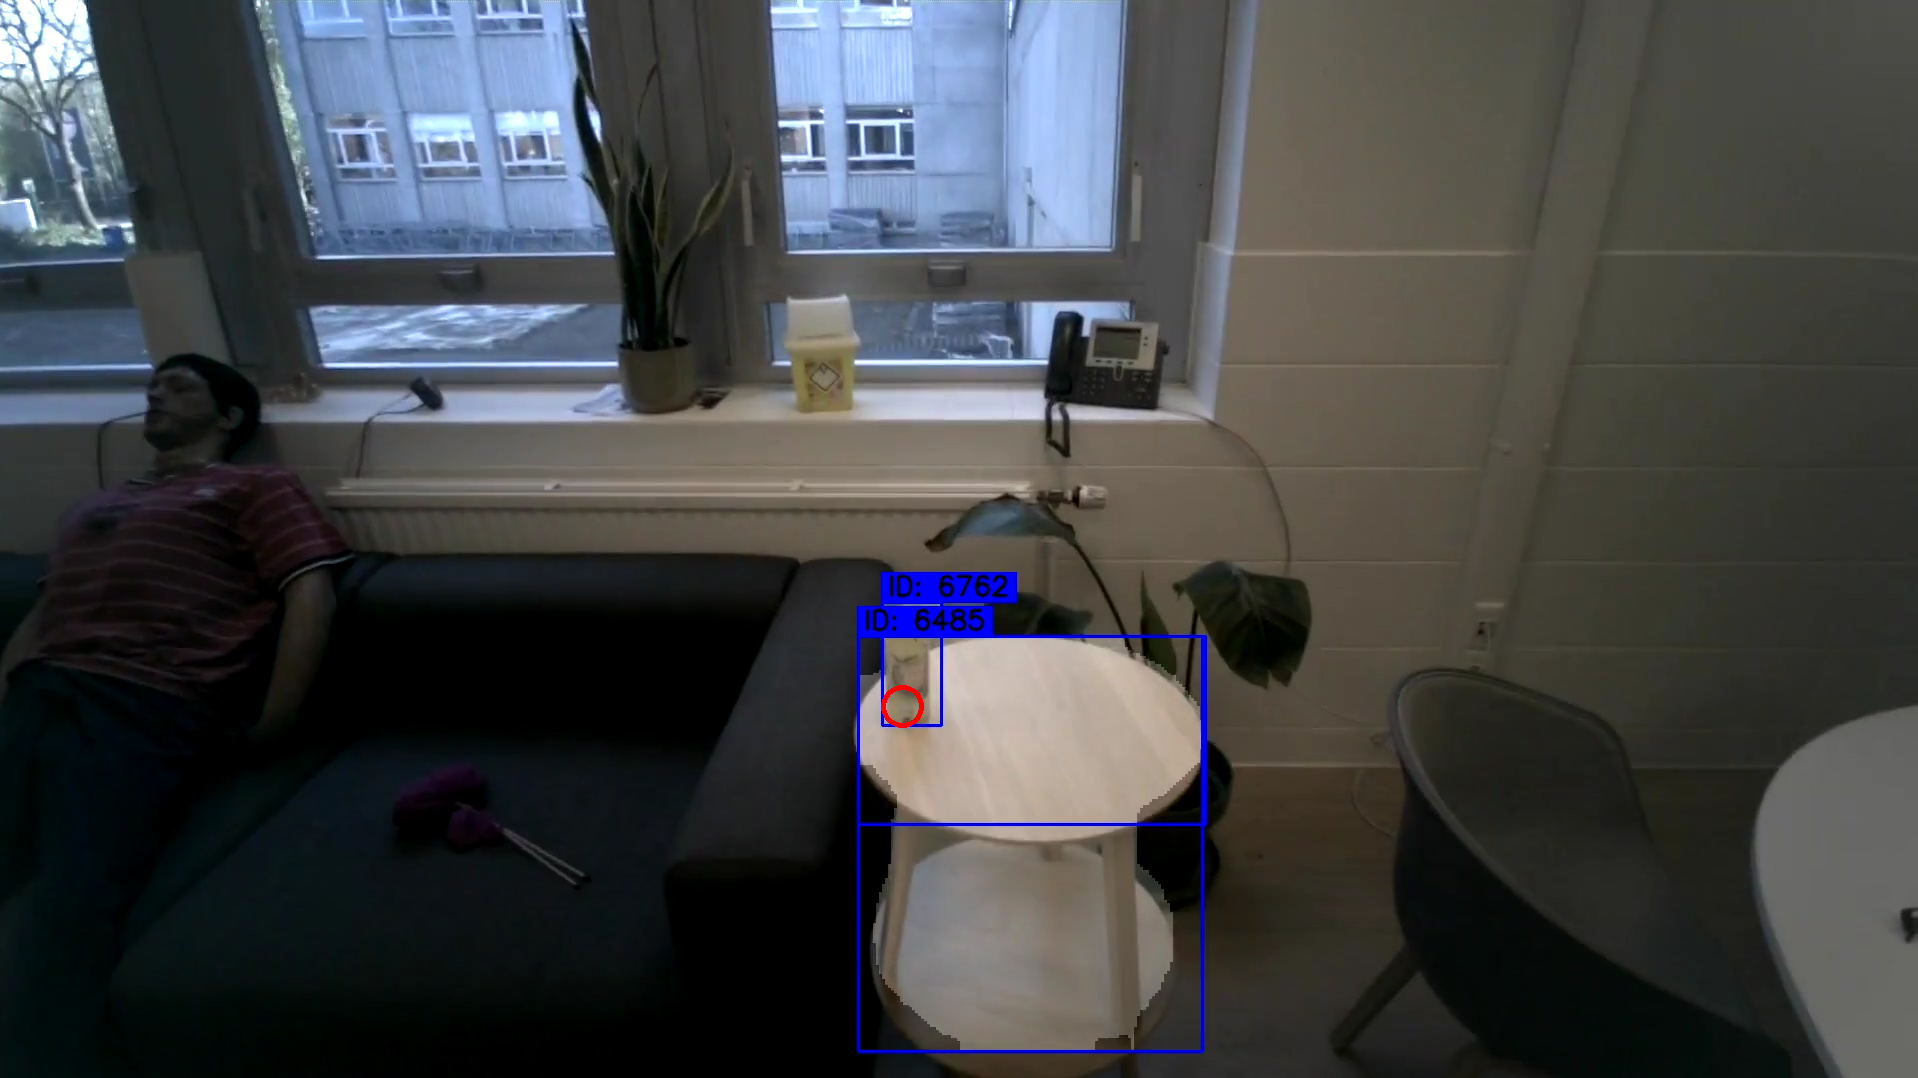
\includegraphics[width=1\textwidth]{filtered-segmentation.png}
    \caption{Filtering op basis van blikpunt en objectgrootte}
    \label{fig:pipeline_stap_b}
    \end{subfigure}

    \vspace{0.5cm}

    \begin{subfigure}[b]{0.75\textwidth}
        \centering
        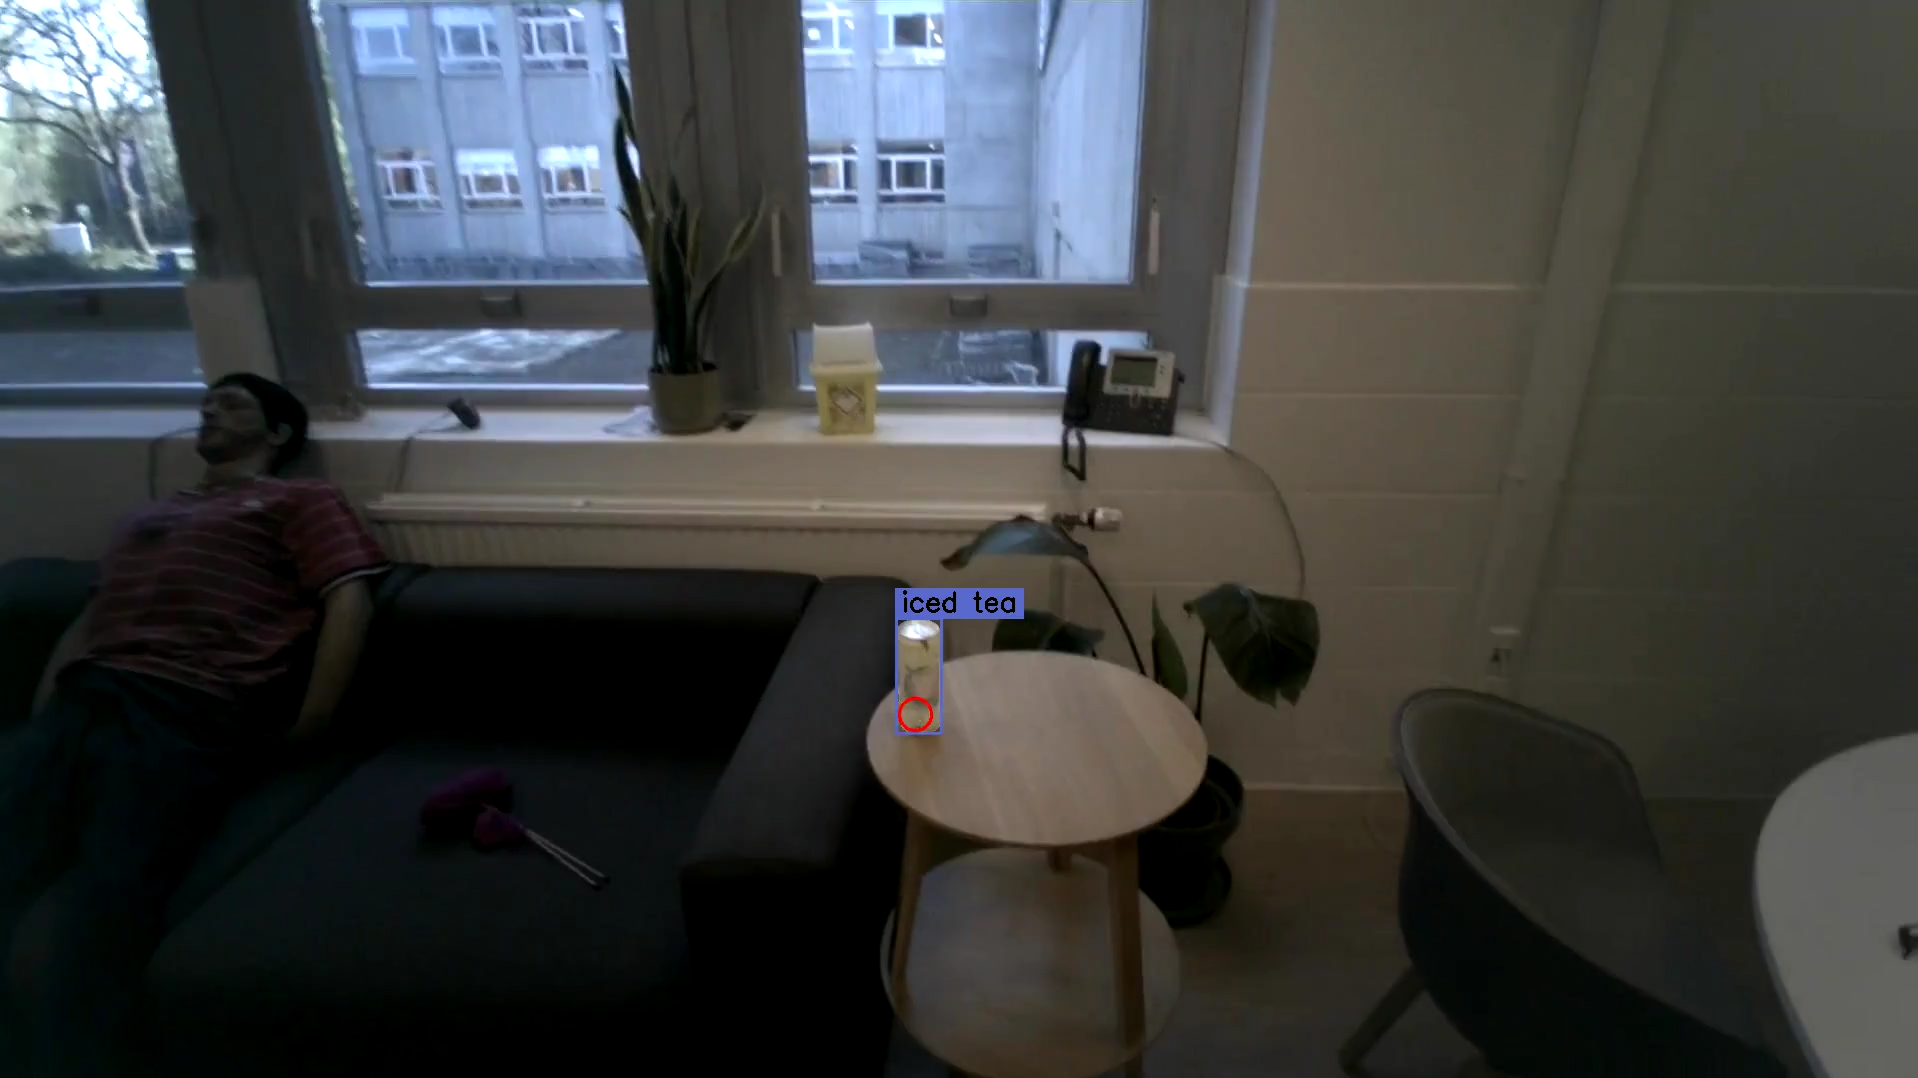
\includegraphics[width=1\textwidth]{classification-example.png}
        \caption{Classificatiestap*}
        \label{fig:pipeline_stap_c}
    \end{subfigure}
    \caption[Visualisatie van de Analysepipeline]{
        \label{fig:analyse-pipeline-visualisatie}
        Visualisatie van de stappen in de analysepipeline.
        (\subref{fig:pipeline_stap_a}) FastSAM identificeert en segmenteert alle potentiële objecten in het frame.
        (\subref{fig:pipeline_stap_b}) De segmenten worden gefilterd; enkel de segmenten die daadwerkelijk met de blik van de gebruiker overlappen worden behouden.
        (\subref{fig:pipeline_stap_c}) De overgebleven segmenten worden uit de originele frame geknipt en dienen als input voor een classificatiemodel.
        *De afbeelding voor de classificatiestap in dit voorbeeld is afkomstig uit een labeling-validatie video.
    }
\end{figure}

\section{Everything-Segmentatie en Objectfiltering}

\section{Classificatie van Objecten}

\subsection{Classificatie met Vector-Index}

\subsection{Classificatie met YOLO}

